%----------------------------------------------------------------------------------------
%	SECTION 2
%----------------------------------------------------------------------------------------
\pagebreak
\section{State Of The Art}



\subsection{Running/hopping model}
Starting with \cite{Blickhan1989} a running/hopping model is analysed. In this model a spring-mass system is introduced by connecting the Center of Mass (CoM) to a massless spring that can describe the dependency of the different physical variables that charecterize running/hopping. Hopping forward can be described by a non-linear system of equations described by an inverted pendulum spring propagating forward in which there are two phases, the ground phase,
\begin{equation}
  \ddot{x}=x\omega^2\left(\frac{l}{\sqrt{x^2+y^2}}-1\right),
\end{equation}
\begin{equation}
  \ddot{y}=y\omega^2\left(\frac{l}{\sqrt{x^2+y^2}}-1\right)-g,
\end{equation}
and the aerial phase, where,
\begin{equation}
  \ddot{x}=0,
\end{equation}
\begin{equation}
  \ddot{y}=-g.
  \end{equation}
\noindent In this system, $m$ is the mass, $\omega^2=\frac{k}{m}$ is the natural frequency of the spring, $g$ is the gravitational acceleration, $x$ is the horizontal displacement, $y$ is the vertical displacement and $l=\sqrt{x_0^2+y_0^2}$ is the rest length of the spring.

\noindent Fig. (\ref{blickhan_model}) helps to illustrate the model presented. In this figure, the mass touches the ground, starting the ground phase, with an angle of atack $\alpha$, with an initial velocity $\vec{v}$ where $\beta$ is the angle that the velocity makes with the ground. After the spring touches the ground, it is compressed in the normal direction, and there is a propagation to the movement of the mass forward becouse the spring rotates around it's pivot point in the ground. After the spring reaches the same height as when it first touched the ground, it starts the aerial phase where the spring becomes disconnected from the ground until the mass reaches an height of $l \cos{\alpha}$ restarting the ground phase.  

\begin{figure}[H]
  \centering
  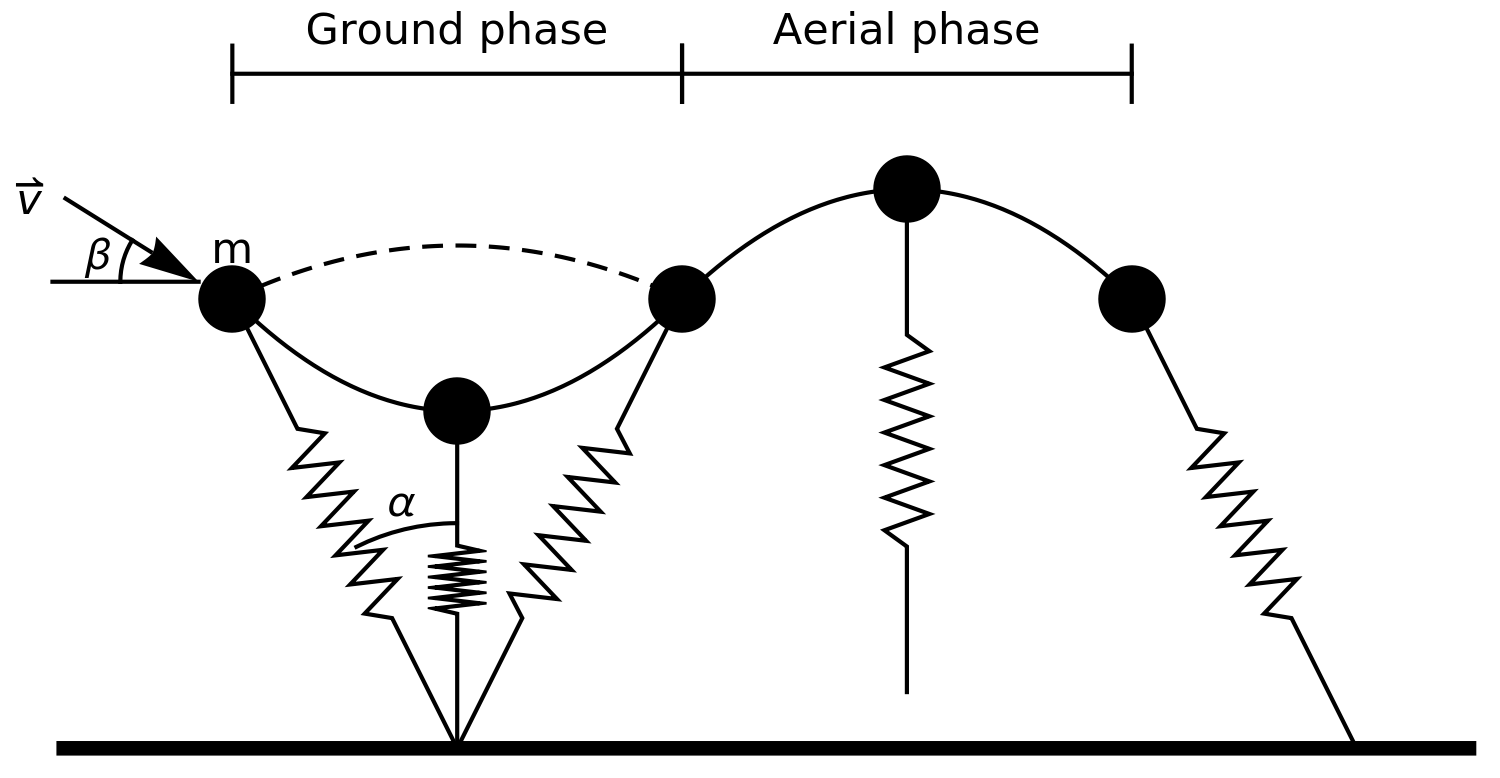
\includegraphics[width=0.7\textwidth]{Blickhan_model}
  \caption{caption}
  \label{blickhan_model}
 \end{figure}

\noindent The determination of the physical solutions are determined by narrowing the range of the parameters studied within the set of possible solutions. With this parameters, we need a small subset of them, the vector of landing velocity and leg length in this model to determine the state of the system and it's evolution.Since this is a physiological model, some of the parameters cannot be changed. An human subject maximizes the amount of energy that can be stored and delivered elastically \cite{Blickhan1989}. This can be achieved by maximizing the contact length and this is why animals use flat angles on the landing velocities.

\subsection{Walking model}

Analysing \cite{Seyfarth:2008}, a model of two compliant legs is proposed. In this model, when one leg is on the ground, the system is equivalent to a inverted spring pendulum,  besides single support, this model also contemplates double support, where the two springs in this phase influence the movement of the CoM in reproducing a bipedal spring-mass walking. The springs accumulate and deliver energy so that the system remains convervative with no energy losses.

\noindent In single phase support, the dynamics of the center of mass (CoM) is as follows,
\begin{equation}
  \ddot{x}=\frac{F_1}{m}\frac{x-x_{t1}}{l_1},
  \end{equation}
\begin{equation}
  \ddot{y}=\frac{F_1}{m}\frac{y-y_{t1}}{l_1}-g.
\end{equation}
\noindent With double support, the dynamics are different from the previous case since we are in the presence of two springs, this is,
\begin{equation}
 \ddot{x}=\frac{F_1}{m}\frac{x-x_{t1}}{l_1}+\frac{F_2}{m}\frac{x-x_{t2}}{l_2},
  \end{equation}
\begin{equation}
  \ddot{y}=\frac{F_1}{m}\frac{y-y_{t1}}{l_1}+\frac{F_2}{m}\frac{y-y_{t2}}{l_2}-g,
\end{equation}
with $F_i$ being the force applied on the mass by the respective leg,
\begin{equation}
  F_i=k(l_0-l_i)\geq 0 \,\,\,\,\, i=1,2\,,
\end{equation}
$l_0$ is the natural length of the spring, $l_i$ is the respective length,
\begin{equation}
l_i=\sqrt{(x-x_{ti})^2+(y-y_{ti})^2} \,\,\,\,\, i =1,2 \,.
\end{equation}
 $(x,y)$ are the coordinates of the center of mass (CoM), $(x_{ti},y_{ti})$ are the coordenates of the respective toes for the leg 1 and leg 2.
\noindent  Fig. (\ref{Seyfarthmodel}) illustrates the model, single support to double support transitions occur when the center of mass drops to a height of $y \sin{\alpha}$ where $\alpha$ is the angle of attack and the vertical velocity is negative. Double support to single support transitions occur when the spring deflection $l_0 - l_i$ of one of the legs return to 0.

\begin{figure}[H]
\centering
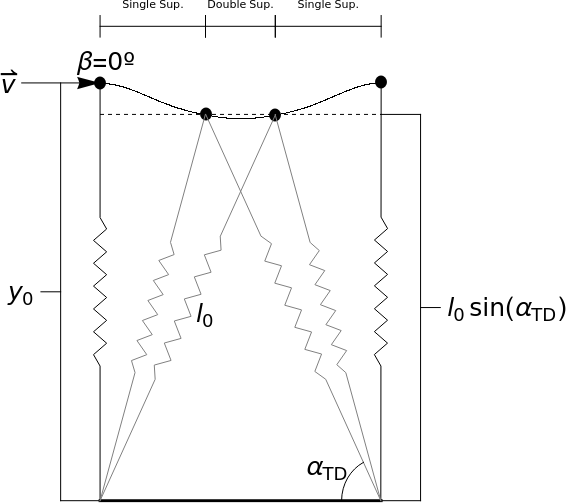
\includegraphics[width=0.7\textwidth]{Seyfarth2006_trimmed.png}
\caption{teste}
\label{Seyfarthmodel}
\end{figure}

Let the Poincare section be defined as the vector $\psi=[y_n,\beta_n]^T$ at the Vertical Leg Orientation (VLO), meaning that everytime the system is in the single support phase and the leg is in it's vertical position we record the vertical position of the CoM $y_n$ and $\beta_n$, the angle that the velocity makes with the ground at this phase and  this defines the step $n$ of the simulation.
\noindent This model is energetically conservative, therefore, the energy $E$ is a constant with,

\begin{equation}
  E=\frac{k (l_0-y_n)^2}{2} + m g y_n + m \frac{v_n^2}{2}.
\end{equation}
\noindent Knowing this, we can express the absolute value of the velocity in terms of the energy. This way, in this model, the only parameters in the initial conditions that can alter the stability of the system for a certain angle of attack $\alpha$, and energy $E$ are $\beta_0$, the angle of the initial velocity with the ground and $y_0$, the initial vertical position of the CoM.

By allowing the simulation to run over one step, we can associate a map, which is called the Poincare map, by defining a function $A$ which iterates the Poincare section, $psi=[y_n,\beta_n]$, this way,

\begin{equation}
  \psi_{n+1}=A \psi_n.
\end{equation}
By recurrence we can apply the $A$ function $n+1$ times from the initial state $\psi_0$ to get to the final step $n+1$.
Not all solutions are admited, if in any instance, the CoM ends up falling this is, $y<0$, or starts walking backwards, $v_x<0$, the set of initial parameters is rejected as a possible stable combination.







